%%%%%%%%%%%%%%%%%%%%%%%%%%%%%%%%%%%% Chapter 

\chapter{La théorie} 	
\label{Chapter1} 		

%%%%%%%%%%%%%%%%%%%%%%%%%%%%%%%%%%%%

%%%%%%%%%%%%%%%%%%%%%%%%%%%%%%%%%%%%%%%%%%%%%%%%%%%%%%%%%%%%%%%%%%%%%%%%%%%%%%%%
%%%%%%%%%%%%%%%%%%%%%%%%%%%%%%%%%%%% SECTION 1 %%%%%%%%%%%%%%%%%%%%%%%%%%%%%%%%%
%%%%%%%%%%%%%%%%%%%%%%%%%%%%%%%%%%%%%%%%%%%%%%%%%%%%%%%%%%%%%%%%%%%%%%%%%%%%%%%%

\section{Regresion de Breukels : théorie 2D} 
\label{sec:Ch1.1}

Si la VSM permet d'étudier l'aérodynamique 3D d'un kite, elle requiert le calcul des coefficients 2D de chaque section($C_L$, $C_D$, $C_M$). Afin de limiter le coût de calcul et de se baser sur des polaires adaptées à des profils "non conventionnels", la VSM utilise une \underline{formule de regression de Breukels}. 

Cette formule est issue de résultats obtenus sur des profils typiques de kites à boudin, et ne \underline{dépend que du diamètre du boudin et de la cambrure du profil}. \\

\begin{center}
    \begin{equation}
        C_L = \lambda_5  \alpha^3 +\lambda_6  \alpha^2 + \lambda_7  \alpha + \lambda_8
        \label{eq:Cl_breukels}
    \end{equation}
\end{center}
avec :
\begin{center}
    \begin{equation}
        \lambda_i = S_x  k + S_y
        \label{eq:lamba_breukels}
    \end{equation}
\end{center}
et :
\begin{center}
    \begin{equation}
        S_i = C_x  t^2 + C_y  t + C_z
        \label{eq:S_breukels}
    \end{equation}
\end{center}
où les 23 coéfficients $C_x$ sont prédéterminés, et (t,k) est le couple (diamètre, cambrure) définit tel que :
\begin{center}
    \begin{equation}
        t = \frac{Diamètre(BA)}{Corde} ; k = \frac{max(CoordonéesExtrados)}{Corde}
        \label{eq:tk_breukels}
    \end{equation}
\end{center}

Ainsi, l'obtention ds coéfficients 2D permet ensuite à la VSM d'ajouter l'indluence des effets 3D (loi de corde, d'envergure, de voute...) sur les coefficients aérodynamiques d'un kite

\begin{figure}[H]
    \centering
    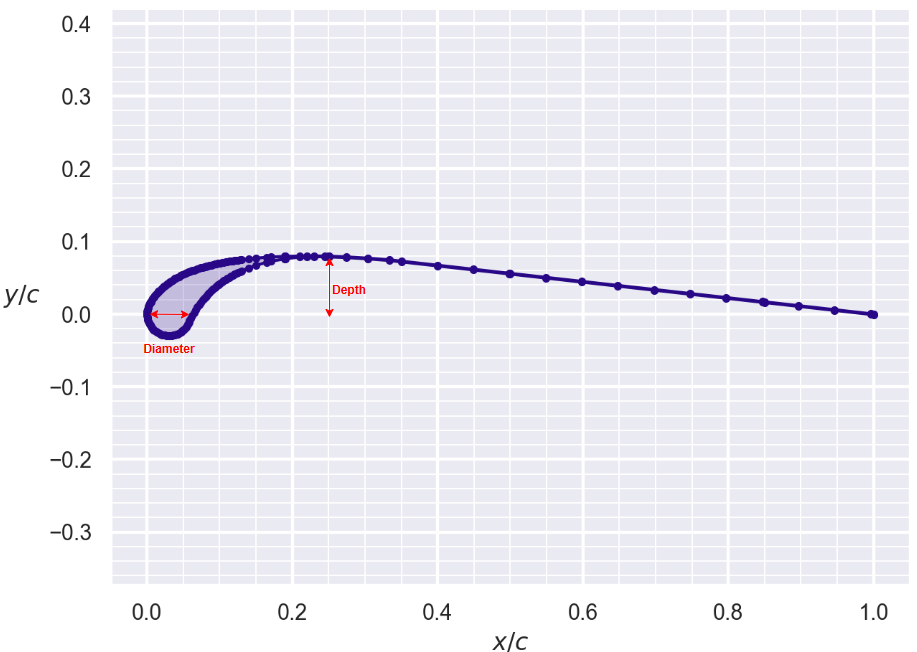
\includegraphics[width=0.5\textwidth]{Pics/01 - La théories/airfoil.png}  
    \caption{Profil central d'une SK50-VG avec identification du diamètre et de la cambrure tel que utilisés par la VSM.}
    \label{fig:airfoil}
\end{figure}